
\documentclass{beamer}


\usetheme{Warsaw}
\usecolortheme{crane}


\title{Fourier Series Fundamentals}
\subtitle{Mathematical Methods in the Physical Sciences}
\author{Steve Mazza}
\institute[Naval Postgraduate School]
{ 
    Naval Postgraduate School \\
    Monterey, CA \\
    
\includegraphics[height=3cm]{images/NPS_logo.jpg}
}
\date {SE3030, Winter/2014 \\ Quantitative Methods of Systems Engineering}
\subject{Quantitative Methods of Systems Engineering}


\begin{document}

\frame{\titlepage}


\frame{{Introduction}
    %TODO
    Fourier series are like power series but are only used to represent periodic functions.
    \begin{center}
        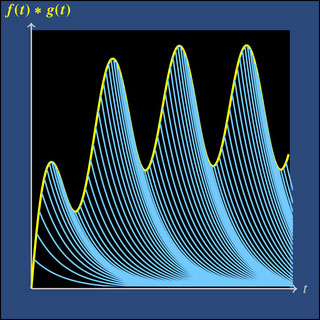
\includegraphics[height=6cm]{images/fourier.jpg}
    \end{center}
}


\frame{{Periodic Functions}
    %TODO
}


\frame{{Applications of Fourier Series}
    %TODO
}


\frame{{Average Value of a Function}
    %TODO
}


\frame{{Fourier Coefficients}
    %TODO
}


\frame{{Dirichlet Conditions}
    %TODO
}


\frame{{Complex Forms of Fourier Series}
    %TODO
}


\frame{{Other Intervals}
    %TODO
}


\begin{frame}{Questions?}
	\begin{center}
		
\includegraphics[width=.7\textwidth]{images/fin.png}
	\end{center}
\end{frame}

\end{document}
